% vim: set tw=78 sts=2 sw=2 ts=8 aw et ai:
\subsection{Computer Vision}

Computer vision is a field that includes methods for acquiring, processing, analyzing, and understanding images and, in general, high-dimensional data from the real world in order to produce numerical or symbolic information, e.g., in the forms of decisions. A theme in the development of this field has been to duplicate the abilities of human vision by electronically perceiving and understanding an image. This image understanding can be seen as the disentangling of symbolic information from image data using models constructed with the aid of geometry, physics, statistics, and learning theory. Computer vision has also been described as the enterprise of automating and integrating a wide range of processes and representations for vision perception.

Applications range from tasks such as industrial machine vision systems which, say, inspect bottles speeding by on a production line, to research into artificial intelligence and computers or robots that can comprehend the world around them. The computer vision and machine vision fields have significant overlap. Computer vision covers the core technology of automated image analysis which is used in many fields. Machine vision usually refers to a process of combining automated image analysis with other methods and technologies to provide automated inspection and robot guidance in industrial applications. As a scientific discipline, computer vision is concerned with the theory behind artificial systems that extract information from images. The image data can take many forms, such as video sequences, views from multiple cameras, or multi-dimensional data from a medical scanner. As a technological discipline, computer vision seeks to apply its theories and models to the construction of computer vision systems. In most practical computer vision applications, the computers are pre-programmed to solve a particular task, but methods based on learning are now becoming increasingly common.

\subsection{Object Category Recognition}

Object recognition in computer vision is the task of finding and identifying objects in an image or video sequence. Humans recognize a multitude of objects in images with little effort, despite the fact that the image of the objects may vary somewhat in different view points, in many different sizes / scale or even when they are translated or rotated. Objects can even be recognized when they are partially obstructed from view. This task is still a challenge for computer vision systems. Many approaches to the task have been implemented over multiple decades.

\begin{figure}[htb]
	\begin{center}
		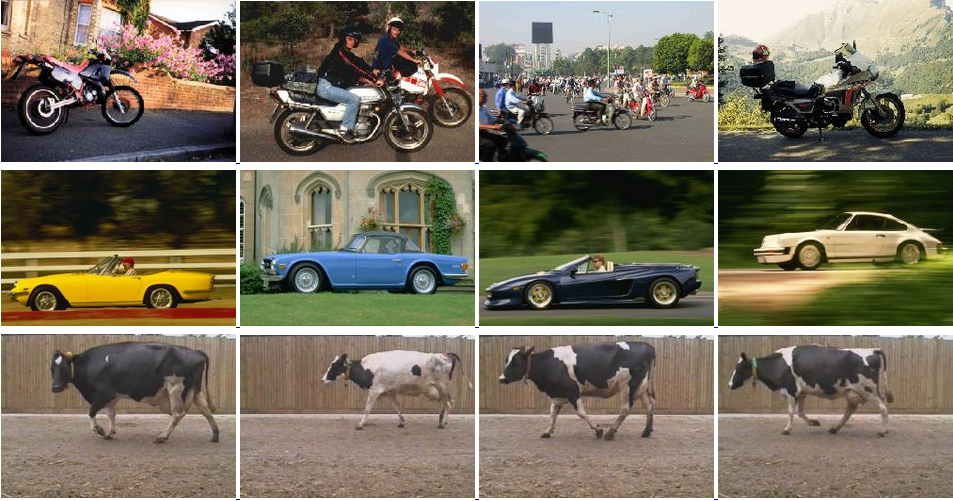
\includegraphics[scale=0.5]{img/objects.png}
	    \caption{Different objects \label{img:objects}}
    \end{center}
\end{figure}


\subsection{Original Work}

The propenents of this method tested their work on human detection. One of the most popular and successful "person detectors" out there right now is the HOG with SVM approach.

HOG stands for Histograms of Oriented Gradients. HOG is a type of "feature descriptor". The intent of a feature descriptor is to generalize the object in such a way that the same object (in this case a person) produces as close as possible to the same feature descriptor when viewed under different conditions. This makes the classification task easier.

The creators of this approach trained a Support Vector Machine (a type of machine learning algorithm for classification), or "SVM", to recognize HOG descriptors of people.

The HOG person detector is fairly simple to understand (compared to SIFT object recognition, for example). One of the main reasons for this is that it uses a "global" feature to describe a person rather than a collection of "local" features. Put simply, this means that the entire person is represented by a single feature vector, as opposed to many feature vectors representing smaller parts of the person.

The HOG person detector uses a sliding detection window which is moved around the image. At each position of the detector window, a HOG descriptor is computed for the detection window. This descriptor is then shown to the trained SVM, which classifies it as either "person" or "not a person".

In our work, we apply this technique on cars photographed from behind.

To recognize cars at different scales, the image is subsampled to multiple sizes. Each of these subsampled images is searched.

The HOG person detector was introduced by Dalal and Triggs at the CVPR conference in 2005. The original paper is available \cite{Dalal05histogramsof}. They used a the INRIA person dataset.

